% langLearnVar 
% Annual Cognitive Science Conference 2016

\documentclass[10pt,letterpaper]{article}

\usepackage{cogsci}
\usepackage{pslatex}
\usepackage{apacite2}
\usepackage{graphicx}
\usepackage{array,multirow}



\newcommand*\rot{\rotatebox{90}}
\newcommand{\squeezeup}{\vspace{-1.5mm}}

\title{Learnability pressures on language across multiple timescales}
\author{{\large \bf Molly Lewis} \\ \texttt{mll@stanford.edu}\\ Department of Psychology \\ Stanford University \\ 
\And {\large \bf Michael C. Frank} \\ \texttt{mcfrank@stanford.edu} \\ Department of Psychology \\ Stanford University \\ }

\begin{document}

\maketitle

\begin{abstract}


\textbf{Keywords:} 
Linguistic Niche Hypothesis; language evolution
\end{abstract}


%%%%% INTRODUCTION %%%%%%
\section{Introduction}
Many facts about the social world are explicable only by considering the broader context: Why do gloves have five fingers? Why do tropical countries use lots of spices? The answers to these questions rely on taking into account properties of individual humans (hands have five fingers), and properties of the broader environmental context  \cite<tropical countries are hot, and spices kill bacteria;>{sherman1999darwinian}. A growing body of work has begun to also explain {\it language structure} by  taking into account these same contextual factors. This work argues that language systems are the product of cognitive constraints internal to the language learner \cite{chater2010language}, as well as properties of the environmental context \cite{nettle2012social} . 

In this paper, we explore this second proposal---that properties of the environmental context shape language systems. This hypothesis, which has been termed the  {\it Linguistic Niche Hypothesis} \cite{lupyan2010language,wray2007consequences}, suggests that language systems adapt to the pressures in the environment where a language is spoken. These pressures may come from a range of sources, including the climate, the length of the growing season, or the demographic characteristics of the people who learn and speak the language. 

An important aspect of this hypothesis is the scale over which these pressures operate \cite{blythe2015hierarchy}. There are at least two scales at which language can be studied: individual utterances, which change over the course of moments in a communicative interaction, and language systems, which change over  the timescale of years.  An established body of work supports the claim  thats speakers adapt to the context at the scale of individual utterances, both in terms of the properties of the listener and the physical environment \cite<e.g.,>{schober1993spatial,frank2012predicting}. The present hypothesis explores the more controversial claim that environmental pressures shape language at the scale of language systems. %2x2 figure?

There are a number of pieces of evidence that environmental factors may indeed shape language systems.  At the lowest level of the linguistic hierarchy, languages with larger populations are claimed to have larger phonemic inventories \cite{atkinson2011phonemic,hay2007phoneme}, but  shorter words \cite{wichmann2011phonological}. Speakers with more second language learners have also been suggested to have fewer lexical items \cite{bentz2015adaptive}. At the level of morphology, evidence suggests that speakers with larger populations tend to have simpler morphology \cite{lupyan2010language, bentz2013languages}. Finally, there is also evidence that population size may influence the mappings between form and meaning. In particular, this work suggests that languages tend to map longer words to more complex meanings \cite{lewisstructure2014}, but that this bias is smaller for languages with larger populations  \cite{lewis_evolang}.

The plausibility of the Linguistic Niche Hypothesis depends largely on the presence of a possible mechanism linking environmental features to aspects of language systems. A range of proposals have been suggested \cite{nettle2012social}. For example, one possibility is that children (L1) and adult (L2) language-learners differ in their learning constraints. In particular, children may be better at acquiring complex morphology than adults, and so languages with mostly children learners may tend to have more complex morphology. A second possibility is that speakers in less dense social networks have less variable linguistic input, and this leads the language system to have more complex morphology.  

%The reported relationships between environmental features and linguistic features described above are efforts to test these hypotheses using available proxies.

Testing these mechanisms is empirically challenging, however. Because there are many factors that shape a linguistic system, large datasets are needed to detect an correlation with environmental factors. In addition, many languages are non-independent because of genetic relationships and language contact, and so data from a wide range of languages are needed to control for these moderators. Third, the scale of this hypothesis makes it difficult to directly intervene on the mechanism. Finally, the hypothesized mechanisms are somewhat underspecified, and the dynamics of these different factors may be complex, trading-off with each other in non-obvious ways \cite<e.g.>{wichmann2011phonological}.

 \begin{figure*}[t]
\begin{center}
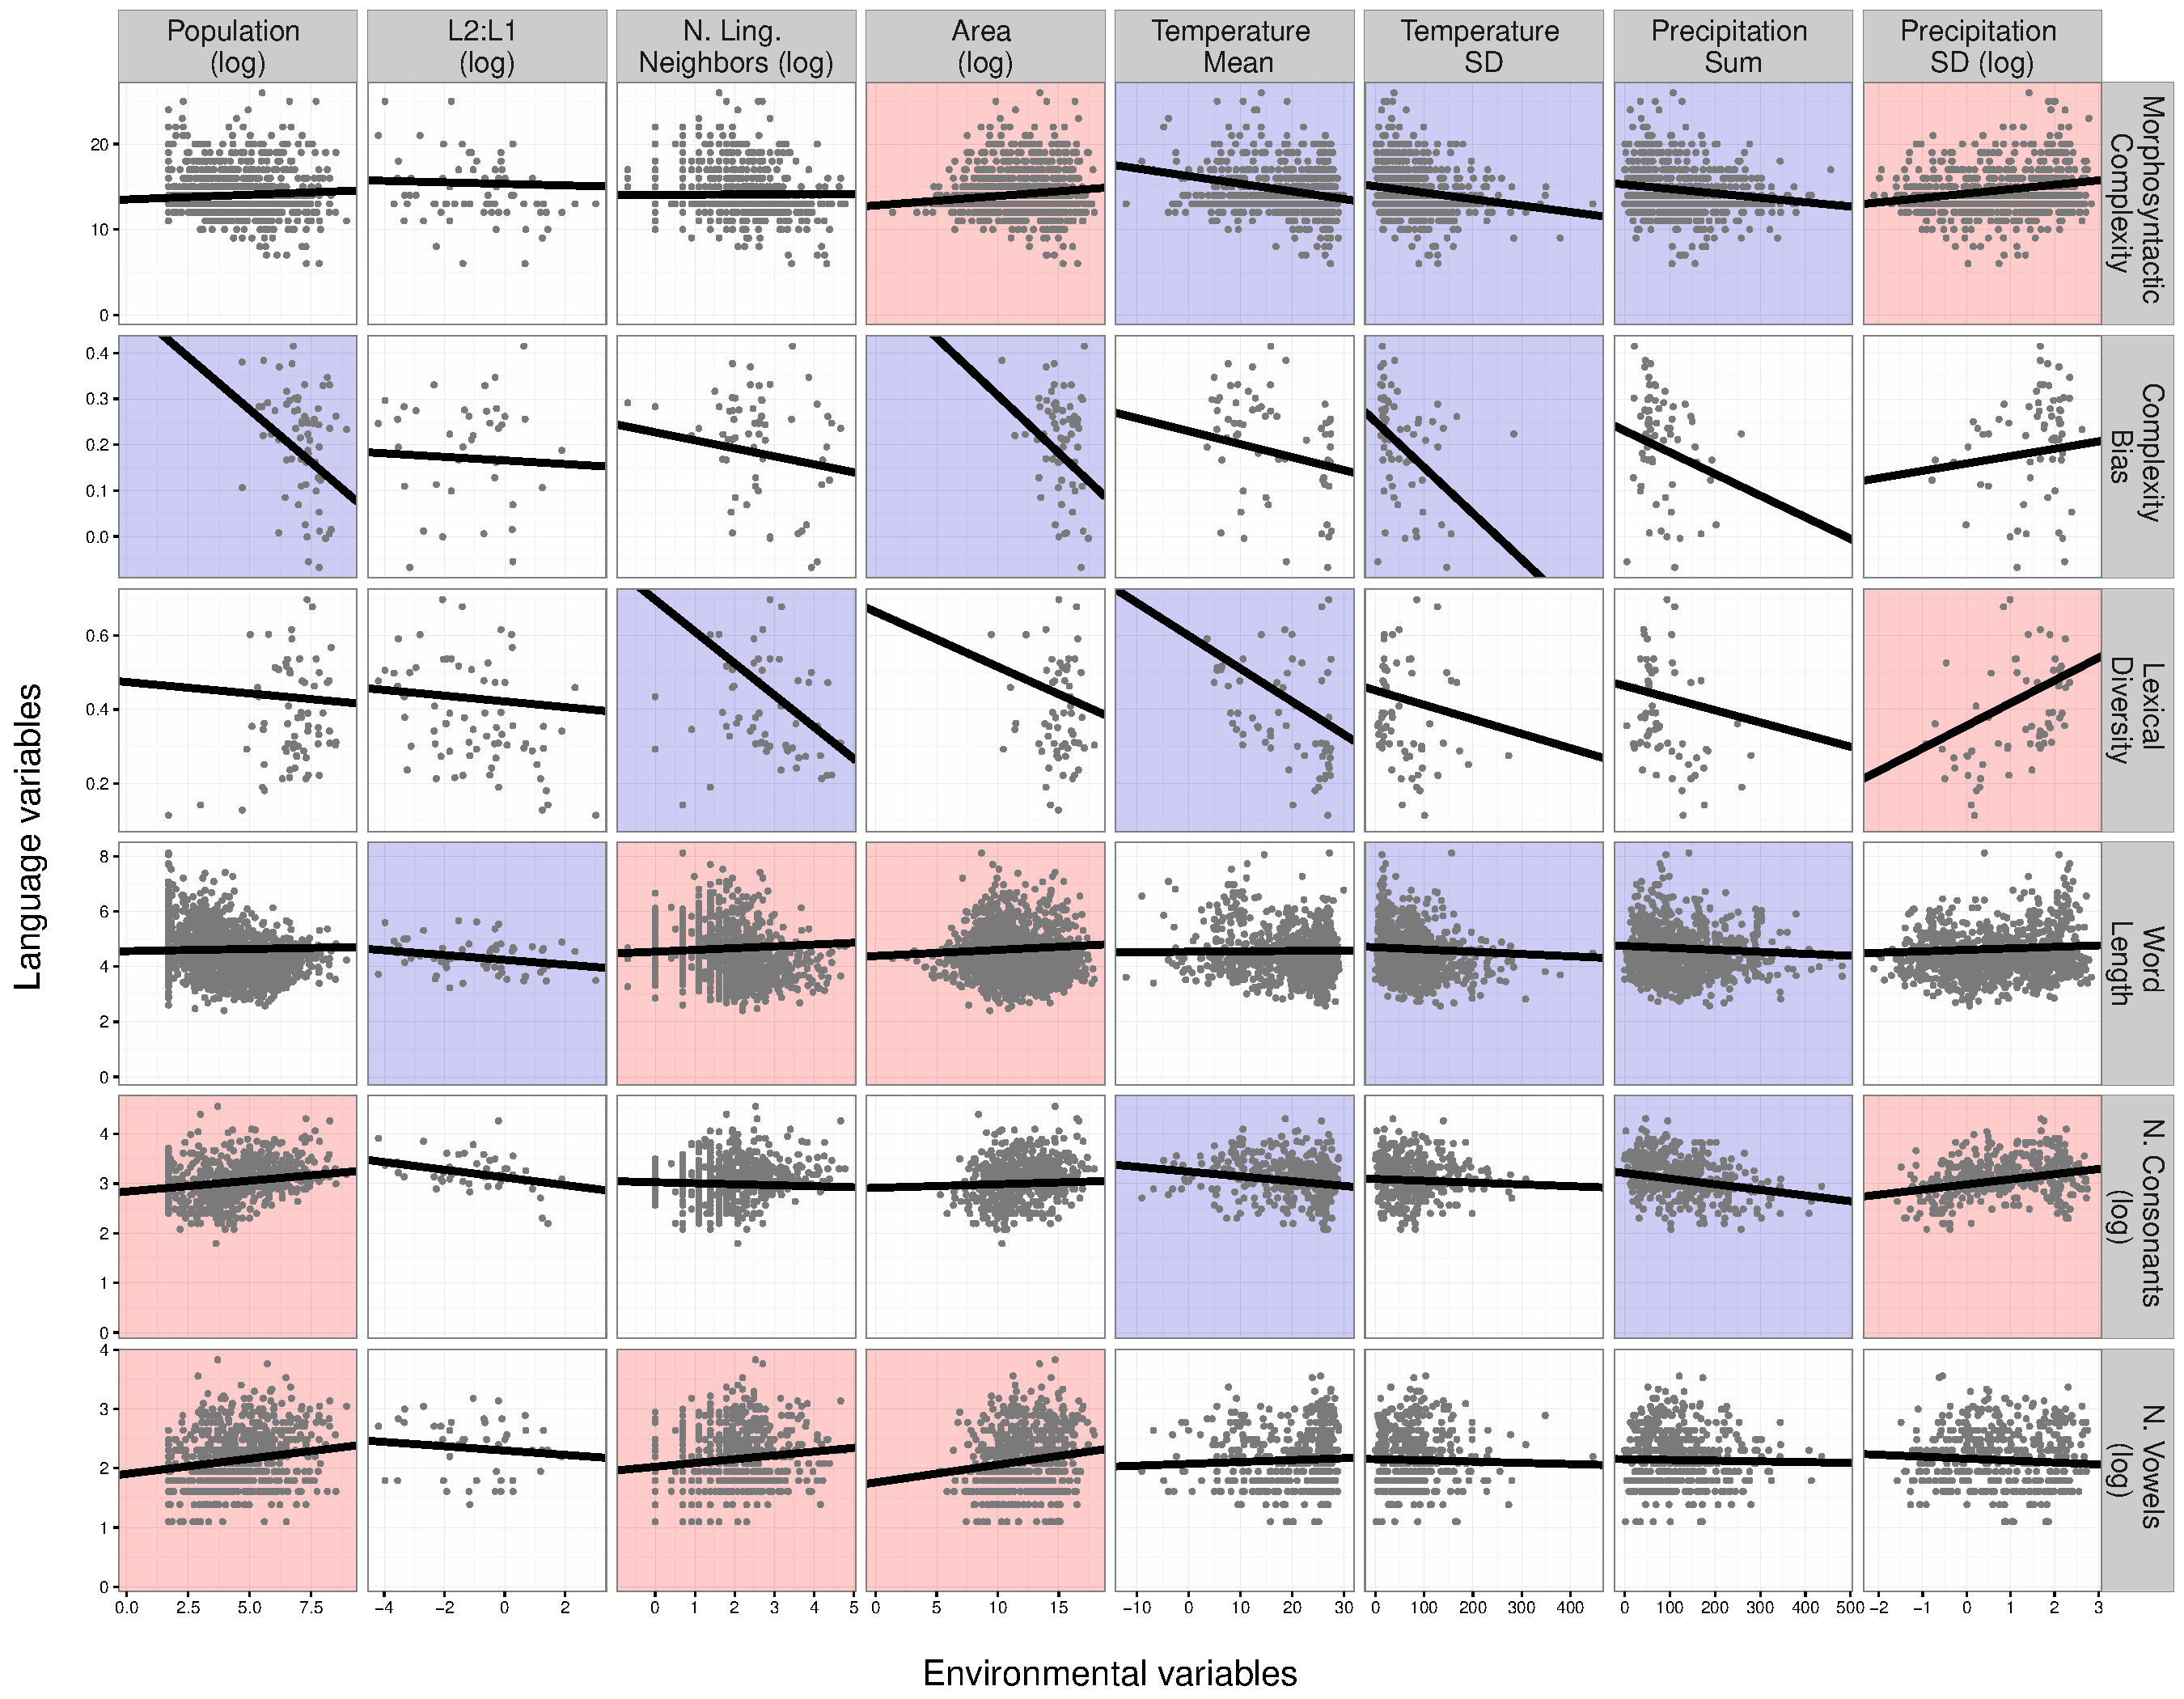
\includegraphics[scale = .4]{figs/plot1.pdf}
\end{center}
\vspace{-.5em}
\caption{Relationship between environmental and linguistic variables, which each point represents a language. Red (positive) and blue (negative) indicate models where the environmental variable is a significant predictor of the linguistic variable. Linear fits are from the fixed effect estimate of the mixed effect model. Number of languages varies across plots due to variation in the number of overlapping languages across datasets.}
\label{fig:cbias}
\vspace{-1em}
\end{figure*}

In this work, we try to address these challenges by clarifying the empirical landscape. We do this by aggregating across datasets that find covariation between environmental variables and linguistic structure. This serves two purposes. First, it allows us to examine the relationship between the same set of environmental predictors across a range of linguistic features. And, second, it allows for the same analytical techniques and areal controls to be used across datasets. By addressing these inconsistencies, we are in a better position to more directly compare relationships between environmental and linguistic features. Importantly, a more coherent picture of the empirical landscape may provide insight into the mechanism linking language systems to their environments.

We also more directly address the question of mechanism by examining variability in the mean age of acquisition of words for L1 learners across languages. Evidence that this variability is related to an aspect of the linguistic system (such as number of phonemes) would suggest that L1 learners, and not L2 learners, are the relevant environmental factor shaping that aspect of the linguistic system. 

In what follows, we first present a set of analyses examining the relationship between environmental and linguistic features using the same analytical techniques.  We then examine the relationship between mean age of acquisition in a language and aspects of the linguistic system.



%%%% Demo and language features%%%%%%
\section{Environmental pressures on language systems}
The hypothesis of interest suggests a relationship between environmental and linguistic features, though the direction  and magnitude of this relationship varies across the previous literature. To explore this variation, we combined data from five existing datasets that included environmental or linguistic data. The datasets were selected for being publicly available and containing a large sample of languages. Below we describe each of these datasets, followed by our analytical method, and results.

\begin{figure*}[t]
\begin{center}
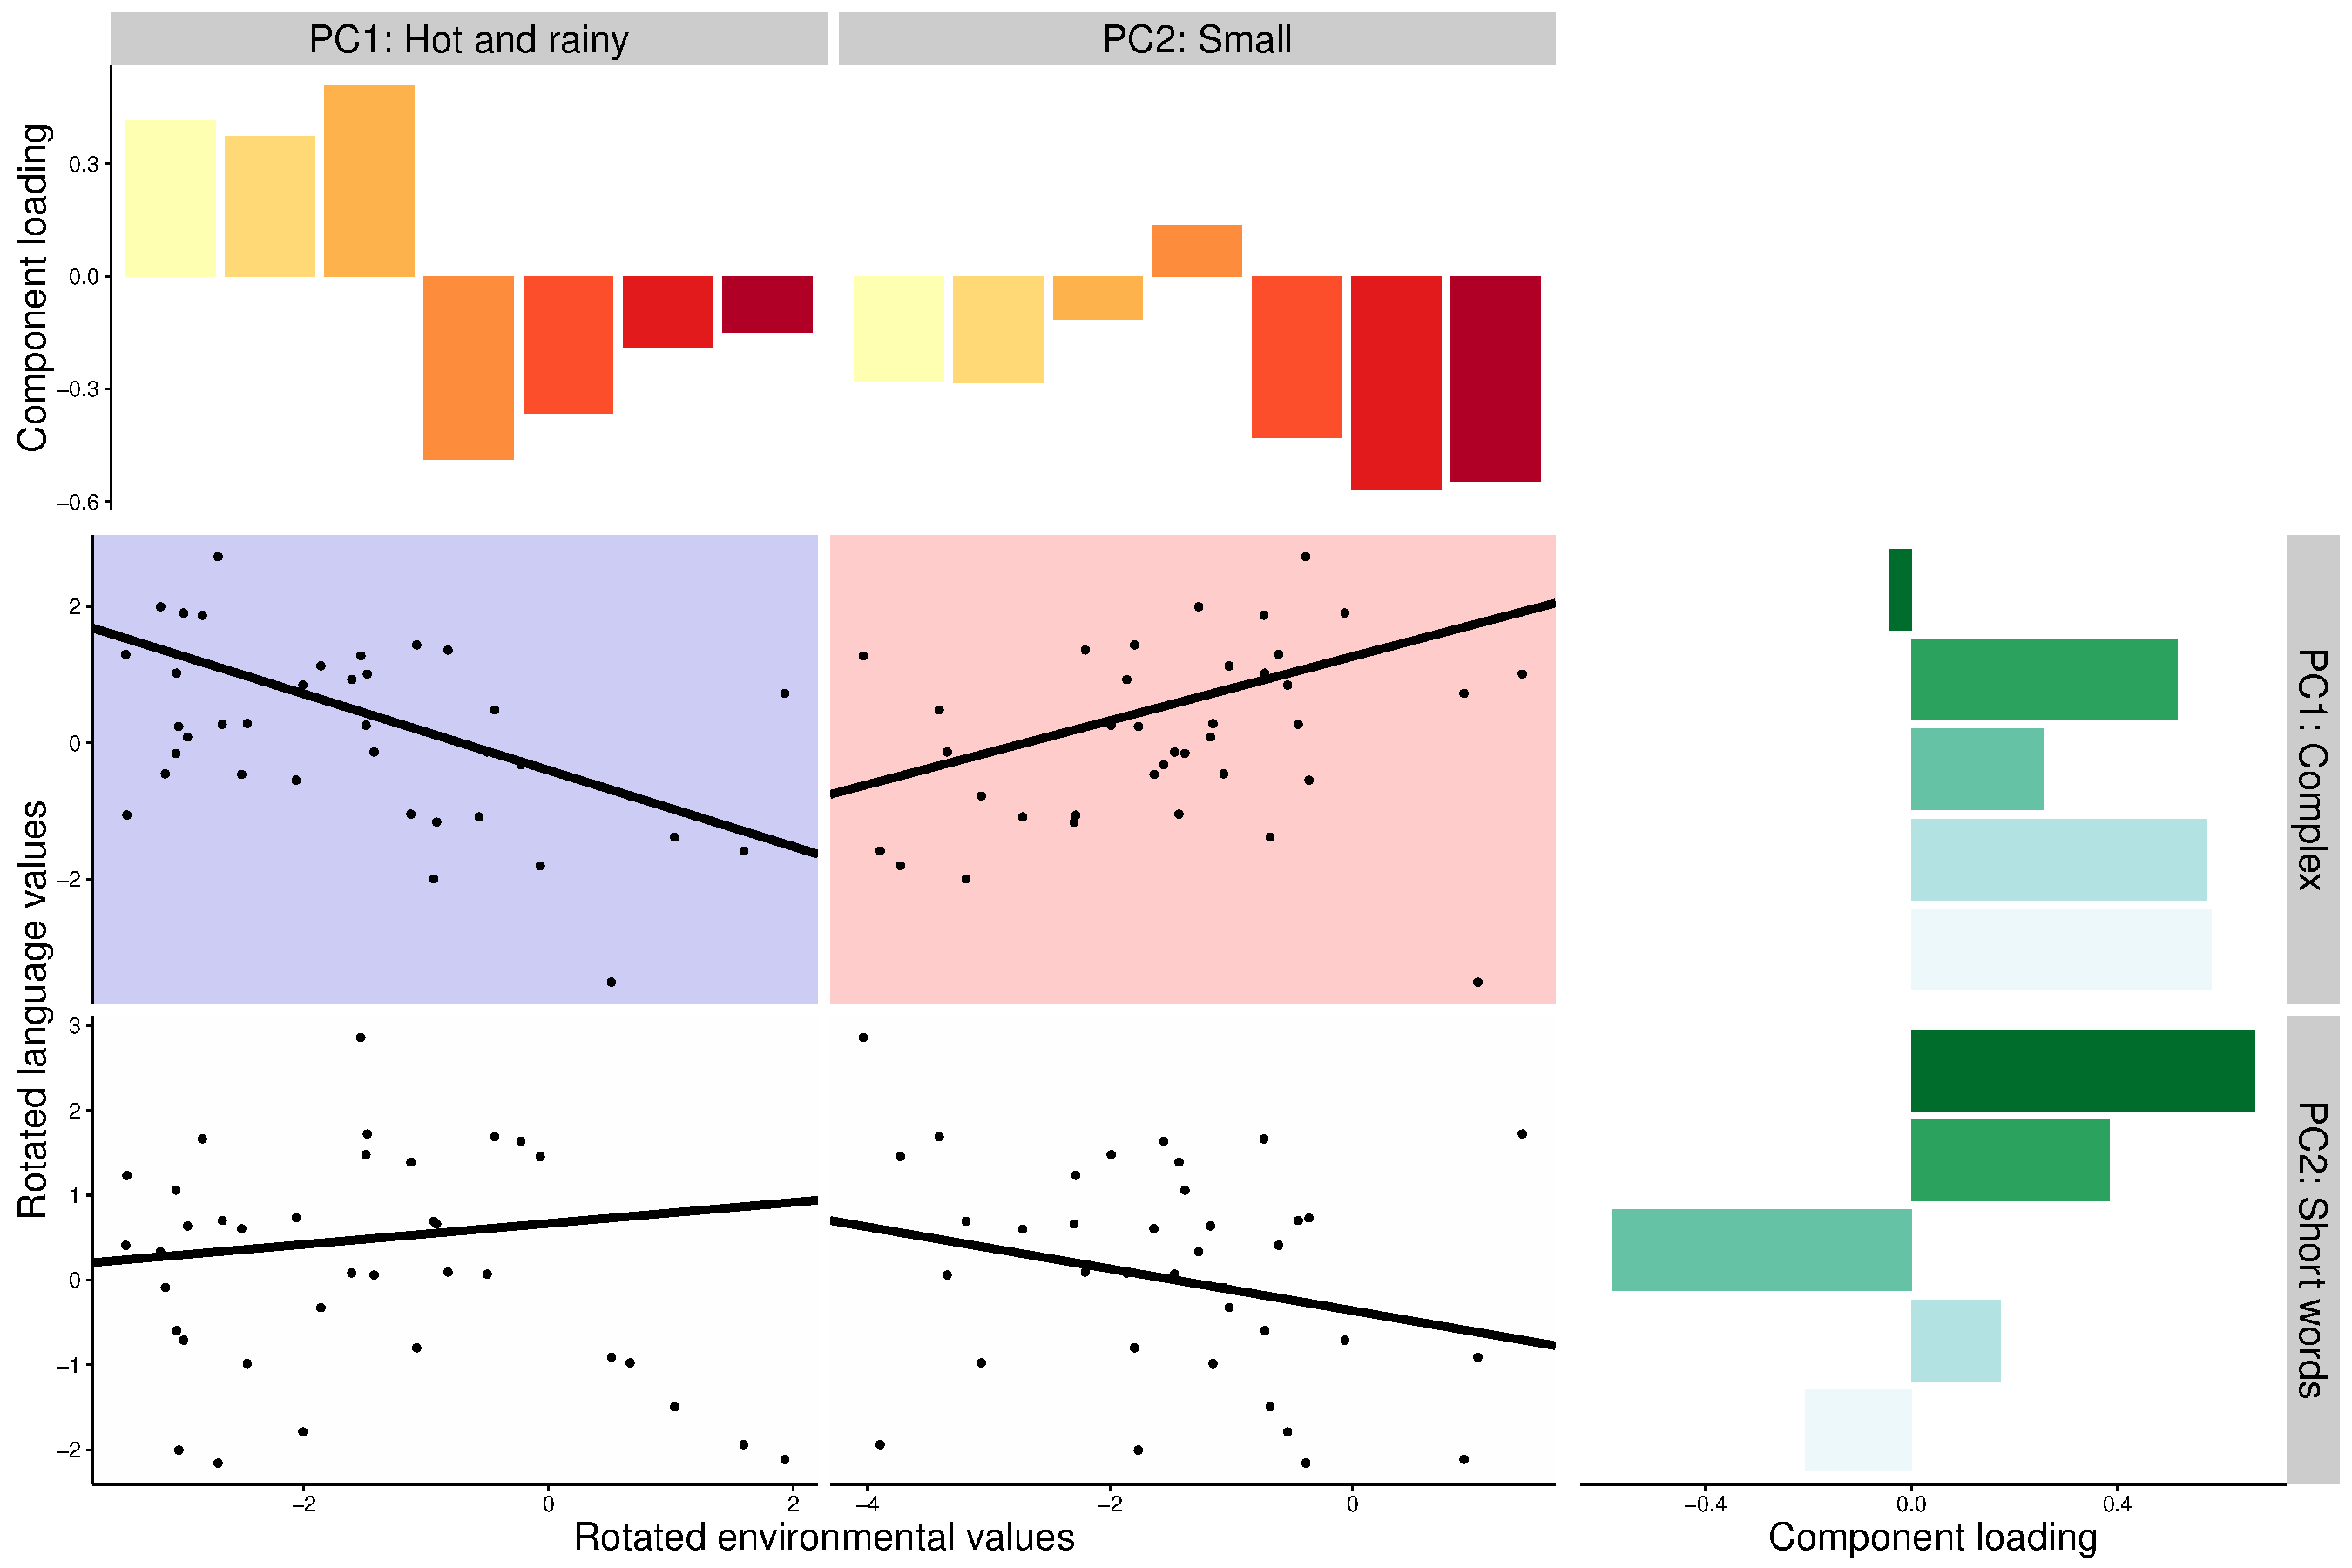
\includegraphics[scale = .35]{figs/plot2.pdf}
\end{center}
\vspace{-.5em}
\caption{Languages in small, cold regions tend to be less complex. The barplots show the loadings on the first two principle components for the environmental variables ($n$ = 7; orange) and language variables ($n$ = 5; green). The scatter plots show the relationship between the first two principle components for both sets of variables. Each point corresponds to a language, and lines show the linear fit from the mixed effect model. Significance and direction of a linear relationship are indicated by the coloring on the scatterplot (red: positive; blue: negative).  [THESE NEEDS A KEY, maybe manually in the upper corner?] }
\label{fig:cbias}
\vspace{-1em}
\end{figure*}

\subsection{Datasets}
{\it Lupyan and Dale (2010).} This dataset contains grammatical information from WALS \cite{wals}, and demographic and geographic information from Ethnologue and the Global Mapping Institute \cite{gordon2005,gmi}. The demographic and geographic variables included total population of speakers, number of neighboring languages, area of region in which the language is spoken ($km$\textsuperscript{2}), mean and standard deviation temperature ($celsius$), and mean and standard deviation precipitation ($cm$). The metric of morphological complexity was calculated from  27 of the 28 morphosyntactic variables\footnote{WALS variable 59 was missing from the dataset.} analyzed in the original paper. For each variable, we coded the strategy as simple if it relied on a lexical strategy or few grammatical distinctions (e.g.,  0-3 noun cases), and complex if it relied on a morphological strategy or many grammatical distinctions (e.g.,  more than 3 noun cases). We summed the number of complex strategies to derive a measure of morphosyntactic complexity measure for each language, including only languages with data for all 27 variables. [$n$ = 1991] 

{\it Bentz et al.\ (2015).} Two variables were used from this dataset: ratio of L2 to L1 speakers and number of word forms. Estimates of number of word forms were taken from translations of  {\it Universal Declaration of Human Rights}. Number of word forms was calculated as the number of unique words divided by the number of total words (type-token ratio). Higher type-token ratio indicates more word types in that language. Speaker population data were taken from a variety of sources, where L2 speakers were restricted to adult non-native speakers only. [$n$ = 81]

{\it Moran, McCloy and Wright (2012).} Estimates of number of consonants and vowels in each language were used from this dataset. These were originally taken from the Phoible database \cite{phoible}. [$n$ = 969]


{\it Lewis and Frank (2014).} This work finds that languages tend to map more complex meanings (measured via semantic norms) to longer words. The bias is estimated as the correlation (Pearson's $r$) between word length (in terms of number of characters) and complexity ratings for a set of 499 words translated via Google Translate. We used estimates of the correlation that partialed out the effect of spoken frequency [$n$ = 79]

{\it Wichmann, Rama, and Holman (2014).} This database contains translations for 40-lexical items across many languages. Word length was calculated as the mean number of characters ASJPcode transcription system across words in each language. [$n$ = 4421]

Aggregating across datasets, we analyzed 8 environmental variables in total: L2-L1 population ratio, total population size, number of neighbors, area of spoken region, mean and standard deviation temperature, and mean and standard deviation precipitation. We analyzed 6 total linguistic variables: number of vowels, number of consonants, word length, type-token ratio, complexity bias, and morphological complexity.








\subsection{Method}
We test for a linear relationship between each environmental and language variable.  A significant challenge in making inferences about language data is non-independence. This non-independence can come from at least two sources: genetic relatedness and language contact. Following \citeA{jaeger2011mixed}, we control for these factors statistically by using linear mixed-effects regression. We control for genetic non-independence by including a random intercept and slope by language family. We control for language contact by including country of origin as a random intercept (models with random slopes failed to converge). While not ideal, we selected country of origin as a proxy for linguistic community because it  was available for all languages in our dataset. Both language family and country of origin were taken from the WALS dataset.\footnote{The model specification was as follows:  \texttt{language.variable $\sim$ environmental.variable + (environmental.variable~\textbar~language.family) +  (1~\textbar~origin.country)}.} 

\subsection{Results}
In our first analysis, we fit mixed effects models predicting language variables with environmental factors using areal controls. In Analysis 2, we reduce the dimensionality of our data using principle component analysis, and then fit the same models as in Analysis 1.

{\it Analysis 1: Relationship between environmental pressures and language systems with areal controls.}
We  log-transformed five of our variables to better approximate a normal distribution (population, L2 to L1 ratio,  number of neighbors, area, number of consonants, number of vowels). We then fit mixed effect models predicting each language variable with each environmental variable. We considered a relationship significant if the test statistic on the fixed effect coefficient exceeded 1.96. Fig. 1 summarizes the results.
[Discussion of findings]

{\it Analysis 2: Principle component analysis.} 
Analysis 1 provides a uniform analysis of the many environmental and linguistic variables that have been used to test the Linguistic Niche Hypothesis. However,  the number of variables considered makes it difficult to distill a coherent picture from these data. Given that many of these variables  are partially correlated with each other, we used a technique for reducing the dimensionality of the dataset---principle component analysis. We found the principle components associated with the variance for the environmental variables and the linguistic variables, and then examined the relationship between the rotated component variables.

All variables were first scaled. For the environmental variables, the first two principle components accounted for  .69 of the total variance (PC1: .39; PC2: .30).  The weights on these variables across the two components can be seen in the upper panel of Fig. 2. The first component  weights most heavily on variables related to the climate. It can be thought of as corresponding to hot and wet regions. The second component weights most heavily on variables related to the size of the region a language is spoken in, both in terms of number of speakers and physical size. This principle component can be roughly interpreted as the `smallness' of a linguistic community.

For the linguistic variables, the first two components also accounted for most of the variance, .70 (PC1: .39; PC2: .31; right panel of Fig.\ 2). The first component weights positively on all variables, except number of vowels. In particular, this component is associated with more consonants, longer words, more word types, and greater morphosyntactic complexity. Broadly, this component is related to the amount of cognitive difficulty associated with learning a language. The second component is associated with having short words, but large phonemic inventories. 

We then fit the same model as in Analysis 1,  using the rotated values for the first two principle components for the environmental and linguistic variables. The plots in Fig.\ 2, show the relationship between the principle components. Both environmental principle components were reliable predictors of the first linguistic principle component (PC1: $\beta=-0.56$; PC2: $\beta=0.47$). This suggests that languages that tend to be  spoken in cold and small regions are more likely to have more complex languages. Neither of the enviromental principle components were reliable predicts of the second linguistic principle component.


\subsection{Discussion}



%%%% AOA %%%%%%
\section{L1 learning and language systems}
\cite{luniewska2015ratings}

% of the linguistic system. If languages with certain Evidence for a relationship for L1 learners would be suggestive that the cognitive constraints of the 

\section{Discussion and Conclusion}

 Other work has empirical + modeling
Some attempts
\cite{silvey2015word}
\cite{perfors2011language}




\cite{wichmann2011phonological}
\cite{wichmann2008languagephonological}
\cite{smith2010eliminating}
\cite{slobin1982children}

\cite{sapir1912language}
\cite{reali2014paradox}


\cite{lupyanrole}\cite{lupyan2010language}
%This proposal is relatively uncontroversial at the level of semantics \cite{sapir}: Languages have words for meanings that are relevant for their environment (e.g. ). But, at  more abstract levels of language structure, this hypothesis has been very controversial. 
\cite{kirby2008cumulative}
Meaning. \cite{silvey2015word}
\cite{perfors2011language}
Critically, 



%\squeezeup


\section{Acknowledgments}
We would like to thank Gary Lupyan and Rick Dale for sharing their data with us.


\bibliographystyle{apacite}

\setlength{\bibleftmargin}{.125in}
\setlength{\bibindent}{-\bibleftmargin}

\bibliography{biblibrary}
\end{document}
